\graphicspath{{chapters/15/images}}
\chapter{Protein motions}

\section{Elastic network models}

\begin{figure}[H]
	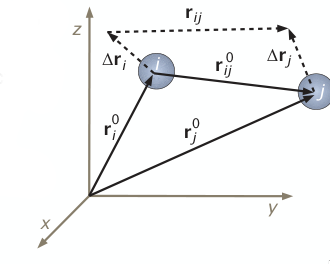
\includegraphics[width=\textwidth]{enm-theory}
	\caption{Elastic network models}
	\label{fig:kirchhoff-adjacency}
\end{figure}

Configuration vector of the protein: $\vec{r} = [\vec{r}_1, \vec{r}_2, \dots, \vec{r}_N]$.
Deviation from the equilibrium position (PDB structure):

$$\Delta\vec{r}_i = \vec{r}_i-\vec{r}_i^0$$

Instantaneous changes in the positions of all residues:

$$\Delta\vec{r} = [\Delta\vec{r}_1, \Delta\vec{r}_2, \dots, \Delta\vec{r}_N]$$


Equilibrium separation between two beads $i$ and $j$: $\vec{r}_{ij}^0 = \vec{r}_j^0-\vec{r}_i^0$.
Instantaneous separation between two beads $i$ and $j$: $\vec{r}_{ij} = \vec{r}_{ij}^0+\Delta\vec{r}_{ij}$, $\Delta\vec{r}_{ij} = \Delta\vec{r}_i-\Delta\vec{r}_i$.

\section{Gaussian network model}
Potential energy for each couple:

$$U_{ij} = \gamma_{ij}(\Delta\vec{r}_j-\Delta\vec{r}_i)\cdot(\Delta\vec{r}_j-\Delta\vec{r}_i) = \gamma_{ij}\Delta\vec{r}_{ij}^2$$

Total elastic energy:

$$U_{GNM} = \frac{1}{2}\sum\limits_i\sum\limits_j\gamma_{ij}\Delta\vec{r}^2_{ij} = \frac{\gamma}{2}\sum\limits_i\sum\limits_j\Delta\vec{r}_{ij}^2$$

Cutoff radius: $r_c = \si{\angstrom}$.

So the total potential energy:

$$U_{GNM} = \frac{\gamma}{2}\Delta\vec{r}(t)^T\Gamma\Delta\vec{r}(t)$$

Where $\Gamma$ is the Kirchoff adjacency matrix.

\begin{figure}[H]
	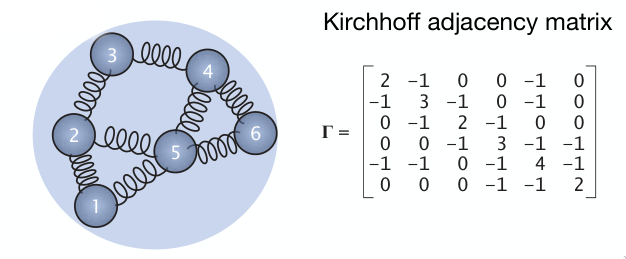
\includegraphics[width=\textwidth]{kirchoff-adjacency-matrix}
	\caption{Kirchhoff adjacency matrix}
	\label{fig:kirchhoff-adjacency}
\end{figure}

	\subsection{Correlated motions}

	$$\langle\Delta\vec{r}_i\cdot\Delta\vec{r}_j\rangle = \frac{1}{Q}\int\Delta\vec{r}_i\cdot\Delta\vec{r}_je^{-\frac{U}{kT}}d^N\Delta\vec{r}$$

	Generalized Gaussian integral:

	$$\langle\Delta\vec{r}_i\cdot\Delta\vec{r}_j\rangle = \frac{3kT}{\gamma}[\Gamma^{-1}]_{ij}$$

	Where $\Gamma^{-1}$ is a pseudoinverse matrix as the Kirchhoff matrix has zero determinant and cannot be inverted.
	Considering the eigenvalue decomposition: $\Gamma = U\Lambda U^T$:

	$$U = [\vec{u}_1, \dots, \vec{u}_{N_1}] = \begin{bmatrix} u_{1,1} & \cdots & u_{N-1,1}\\\vdots & \cdots & \vdots\\ u_{1, N} & \cdots & u_{N-1, N}\end{bmatrix}\qquad\Lambda = \begin{bmatrix} \lambda_1 & 0 & 0 & \cdots & 0\\ 0 & \lambda_2 & 0 &\cdots & 0\\0 & 0& \lambda_3 & \cdots & 0\\\vdots & \vdots & \vdots & \vdots &\vdots\\ 0 & 0 & 0 & \cdots & \lambda_{N-1}\end{bmatrix}$$

	\subsection{Gaussian network model and B-factors}

	$$\langle\Delta\vec{r}_i\cdot\Delta\vec{r}_i\rangle = \frac{3kT}{\gamma}[U\Lambda^{-1}U^{T}]_{ii} = \frac{3kT}{\gamma}\sum\limits_{k}[\lambda_k^{-1}\vec{u}_k\vec{u}_k^T]_{ii} = \sum\limits_{k}[\Delta r_i^2]_k$$

	Debye-Waller factors:

	$$B_i = \frac{8\pi^2}{3}\langle\Delta r_i^2\rangle$$

	\begin{figure}[H]
		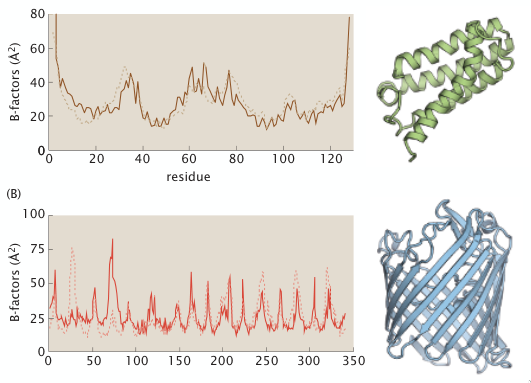
\includegraphics[width=\textwidth]{gnm-b-factors}
		\caption{GNM and B-factors}
		\label{fig:gnn-b-factors}
	\end{figure}

	\subsection{Biological relevance}

	\begin{figure}[H]
		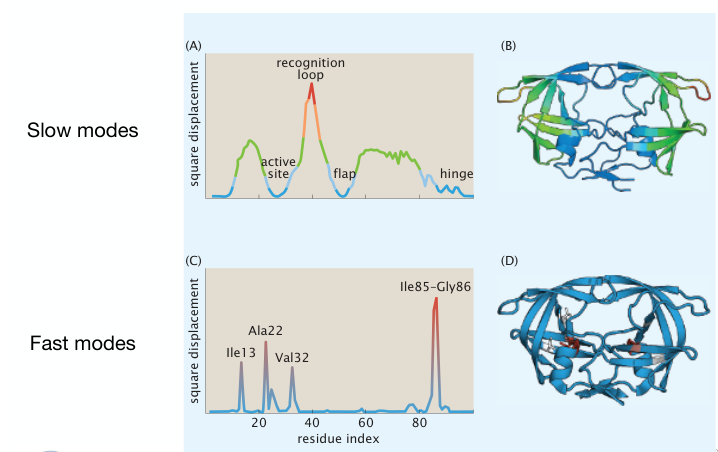
\includegraphics[width=\textwidth]{biological-relevance}
		\caption{Biological relevance}
		\label{fig:biological-relevance}
	\end{figure}

	\subsection{Normal mode analysis}

	$$U = U_0 + \sum\limits_i\frac{\partial U}{\partial q_i}|_{q^0}(q_i-q_i^0) + \frac{1}{2}\sum\limits_i\sum\limits_j\frac{\partial^2 U}{\partial q_i\partial q_j}|_{q^0}(q_i-q_i^0)(q_j-q_j^0) + \cdots$$

	At equilibrium:

	$$U = \frac{1}{2}\Delta\vec{q}^TH\Delta\vec{q} = \frac{1}{2}\sum\limits_i\sum\limits_j H_{ij}(q_i-q_i^0)(q_j-q_j^0)$$

	Hessian matrix:

	$$H_{ij} = \frac{\partial^2 U}{\partial q_i\partial q_j}|_{q^0}$$

	Covariance matrix:

	$$C = \langle\Delta\vec{q}\Delta\vec{q}^T\rangle = \frac{1}{Q}\int\Delta\vec{q}\Delta\vec{q}^Te^{-\frac{\Delta\vec{q}^TH\Delta\vec{q}}{2kT}}d^N\Delta\vec{q} = kTH^{-1}$$
